\documentclass[10pt,twocolumn]{article}

\usepackage[margin=1.8cm]{geometry}
\usepackage{amsmath,amssymb}
\usepackage{graphicx}
\usepackage{booktabs}
\usepackage{hyperref}
\usepackage{tikz}
\usetikzlibrary{shapes,arrows.meta,positioning}

\graphicspath{{figures/}}
\hypersetup{colorlinks=true, linkcolor=blue, citecolor=blue}

\title{\textbf{GPT4RUL Reproduction and Improvement:\\Technical Report on LLM-based RUL Prediction}}
\author{Haoxiang Li}
\date{July 2026}

\begin{document}
\maketitle

%==============================================================================
\section*{Abstract}
%==============================================================================

This report presents an independent reproduction and systematic improvement of GPT4RUL (Tan et al., QR2MSE 2025) on the NASA C-MAPSS benchmark (FD001--FD004).
The pipeline combines KMeans-based normalization, correlation--monotonicity feature selection, Patch-Channel Fusion (PCF) blocks, and a frozen GPT-2 backbone, extended with condition embedding and soft prompts.
Under the reproduced configuration, GPT4RUL+CE achieves test RMSE of 14.87/12.87/13.69/13.38 across four subsets; Hybrid+Soft Prompt reaches \textbf{12.55} on FD002, outperforming the reported paper baseline on that subset.
Ablation studies show that validating on only the last window per engine degrades test RMSE by 5--11 cycles, and random engine-disjoint splits are essential to avoid leakage.
Code and one-click reproduction scripts are available at \url{https://github.com/icemilk-1/GPT4RUL-Reproduction}.

%==============================================================================
\section{Method}
%==============================================================================

\subsection{Preprocessing}

On C-MAPSS, preprocessing proceeds as follows:
\begin{itemize}
  \item \textbf{Regime-aware normalization:} KMeans on three operating settings ($K{=}1$ for FD001/003; $K{=}6$ for FD002/004), per-cluster Z-score, then global MinMax to $[0,1]$.
  \item \textbf{Feature selection:} for sensor $j$,
  \begin{equation}
    Cri_j = 0.5 \cdot |r_j| + 0.5 \cdot mono_j,
  \end{equation}
  keeping sensors with $Cri_j > \bar{Cri}$ (13--14 sensors), plus 3-dim condition embedding (17 features total).
  \item \textbf{Windowing \& split:} stride${=}1$, RUL cap 125; Random Engine Split (80/20 by engine ID) to prevent cross-set leakage.
\end{itemize}

\subsection{Architecture}

Figure~\ref{fig:arch} summarizes GPT4RUL. Given $\mathbf{X} \in \mathbb{R}^{B \times T \times F}$, patching ($K{=}8$) feeds PCF blocks:
\begin{align}
  \mathbf{H}' &= \mathbf{H} + \mathrm{MLP}_{\mathrm{patch}}(\mathrm{LN}(\mathbf{H})), \\
  \mathbf{H}'' &= \mathbf{H}' + \mathrm{MLP}_{\mathrm{channel}}(\mathrm{LN}(\mathbf{H}')),
\end{align}
followed by linear mapping to 768-dim, frozen 3-layer GPT-2, flatten, and RUL head.
Hybrid Prompt RUL prepends $M{=}4$ learnable 768-dim soft prompt tokens.
Only PCF, projections, head (and soft prompts) are trainable; GPT-2 remains frozen ($\sim$38M params).

\begin{table}[t]
  \centering
  \caption{Per-dataset hyperparameters (Tan et al., Table 2).}
  \label{tab:hparams}
  \scriptsize
  \begin{tabular}{@{}lcccc@{}}
    \toprule
    Param & FD001 & FD002 & FD003 & FD004 \\
    \midrule
    Window & 30 & 64 & 40 & 64 \\
    Patch stride & 4 & 8 & 8 & 8 \\
    PCF blocks & 2 & 2 & 1 & 2 \\
    Mixing factor & 2 & 2 & 1 & 1 \\
    Batch size & 64 & 128 & 64 & 128 \\
    \bottomrule
  \end{tabular}
\end{table}

\begin{figure*}[t]
  \centering
  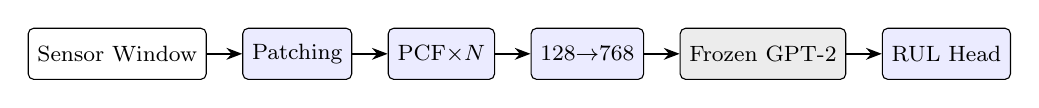
\begin{tikzpicture}[
    node distance=0.4cm and 0.45cm,
    box/.style={rectangle, draw, rounded corners=2pt, minimum height=0.65cm,
                minimum width=1.35cm, align=center, font=\footnotesize},
    trainable/.style={box, fill=blue!8},
    frozen/.style={box, fill=gray!15},
    arrow/.style={-{Stealth[length=2mm]}, thick}
  ]
    \node[box, minimum width=1.8cm] (in) {Sensor Window};
    \node[trainable, right=of in] (patch) {Patching};
    \node[trainable, right=of patch] (pcf) {PCF$\times N$};
    \node[trainable, right=of pcf] (map) {128$\rightarrow$768};
    \node[frozen, right=of map] (gpt) {Frozen GPT-2};
    \node[trainable, right=of gpt] (head) {RUL Head};
    \foreach \a/\b in {in/patch, patch/pcf, pcf/map, map/gpt, gpt/head}
      \draw[arrow] (\a) -- (\b);
  \end{tikzpicture}
  \caption{GPT4RUL architecture (blue: trainable; gray: frozen).}
  \label{fig:arch}
\end{figure*}

\subsection{Training}

Adam ($lr{=}0.005$, weight decay 0.01), MSE loss, dropout 0.2, StepLR ($\times 0.1$ every 10 epochs), early-stop patience${=}10$.
Batch sizes: 64/128/64/128 for FD001--FD004; validation uses all engine-disjoint windows (\texttt{val\_mode=all}).

%==============================================================================
\section{Experiments}
%==============================================================================

PyTorch, seed${=}42$; metrics:
\begin{equation}
  \mathrm{RMSE} = \sqrt{\frac{1}{N}\sum_{i=1}^{N}(\hat{y}_i - y_i)^2},
\end{equation}
and asymmetric C-MAPSS Score; predictions clipped to $[0,125]$.

\begin{table}[t]
  \centering
  \caption{Main reproduction vs.\ Tan et al.\ (2025).}
  \label{tab:main}
  \small
  \begin{tabular}{@{}lccc@{}}
    \toprule
    Dataset & Paper & Reproduced & Gap \\
    \midrule
    FD001 & 11.23 & 14.87 & +3.64 \\
    FD002 & 11.05 & 12.87 & +1.82 \\
    FD003 & 11.45 & 13.69 & +2.24 \\
    FD004 & 12.68 & 13.38 & +0.70 \\
    \bottomrule
  \end{tabular}
\end{table}

\begin{table}[t]
  \centering
  \caption{Multi-model test RMSE comparison (lower is better).}
  \label{tab:models}
  \scriptsize
  \begin{tabular}{@{}lcccc@{}}
    \toprule
    Dataset & PCF only & GPT4RUL+CE & Hybrid+SP & Paper \\
    \midrule
    FD001 & 14.16 & 14.87 & \textbf{13.80} & 11.23 \\
    FD002 & 13.61 & 12.87 & \textbf{12.55} & 11.05 \\
    FD003 & \textbf{12.99} & 13.69 & 13.59 & 11.45 \\
    FD004 & 14.52 & \textbf{13.38} & 13.76 & 12.68 \\
    \bottomrule
  \end{tabular}
\end{table}

Table~\ref{tab:main} reports GPT4RUL+condition embedding; FD004 is closest to the paper (+0.70 RMSE).
Table~\ref{tab:models} compares three variants: PCF-only wins on simple FD003; Hybrid+soft prompts win on multi-regime FD001/002, with \textbf{FD002 (12.55) as the only subset beating the paper baseline among tested configs}.

\begin{figure}[t]
  \centering
  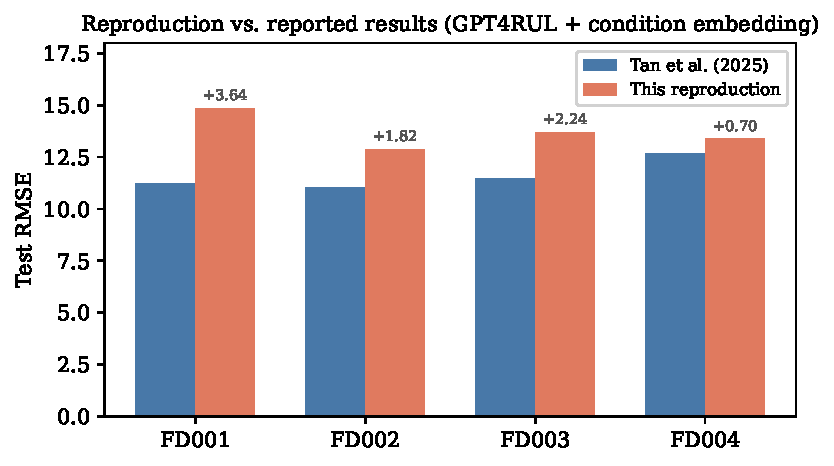
\includegraphics[width=\linewidth]{fig4_rmse_comparison.pdf}
  \caption{Reproduced vs.\ reported RMSE.}
  \label{fig:rmse}
\end{figure}

%==============================================================================
\section{Ablation Findings}
%==============================================================================

\subsection{Validation Protocol Trap}

Using only the last window per engine for validation (RUL$\approx$0) induces a near-zero prediction shortcut, severely degrading test RMSE (Table~\ref{tab:val}).

\begin{table}[t]
  \centering
  \caption{Validation protocol ablation (test RMSE).}
  \label{tab:val}
  \small
  \begin{tabular}{@{}lccc@{}}
    \toprule
    Dataset & last\_window & all-val & Gain \\
    \midrule
    FD001 & 26.19 & 14.87 & $-$11.32 \\
    FD002 & 17.90 & 12.87 & $-$5.03 \\
    FD003 & 23.89 & 13.69 & $-$10.20 \\
    \bottomrule
  \end{tabular}
\end{table}

\begin{figure}[t]
  \centering
  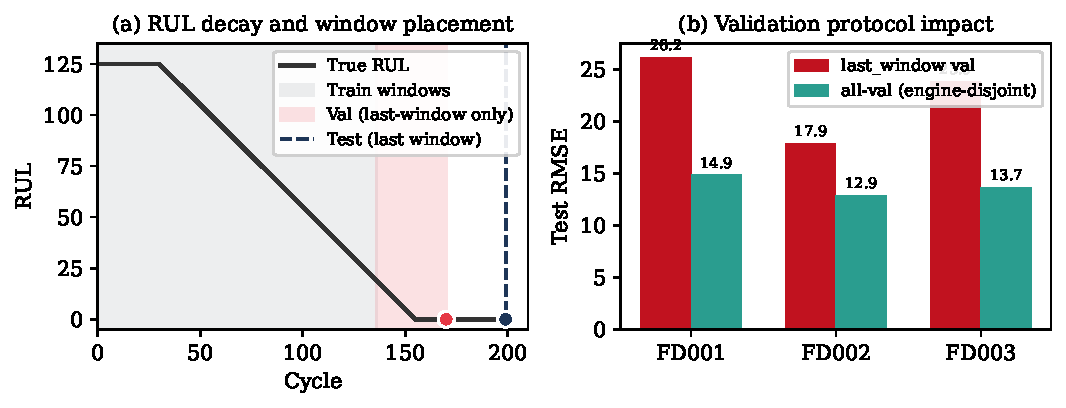
\includegraphics[width=\linewidth]{fig3_validation_trap.pdf}
  \caption{RUL decay and validation protocol impact.}
  \label{fig:valtrap}
\end{figure}

\subsection{Diagnostic Checklist}

\begin{table}[t]
  \centering
  \caption{Selected items from 12+ reproduction diagnostics.}
  \label{tab:diag}
  \scriptsize
  \begin{tabular}{@{}ll@{}}
    \toprule
    Item & Outcome \\
    \midrule
    last\_window $\rightarrow$ all val & +5--11 RMSE gain \\
    Random Engine Split & No leakage (adopted) \\
    Temporal split & val inflated $\sim$6.6 RMSE \\
    Condition Embedding & Improved all 4 subsets \\
    Dual Pre-LN PCF & Aligned with MLP-Mixer \\
    Dropout 0.3 / LR 0.002 & Degraded \\
    Grad clip off vs 1.0 & Preliminary: off better \\
    GPT-2 layer count & Pending ablation \\
    \bottomrule
  \end{tabular}
\end{table}

\textbf{Key findings:}
(1)~LLM value depends on task complexity; PCF-only suffices on simple FD003;
(2)~Soft prompts are critical to activate GPT-2; without them LLM can hurt performance;
(3)~\emph{Evaluation protocol} (split and validation design) matters more than PCF micro-tuning ($<0.5$ RMSE);
(4)~No single architecture wins on all four subsets.

\begin{figure}[t]
  \centering
  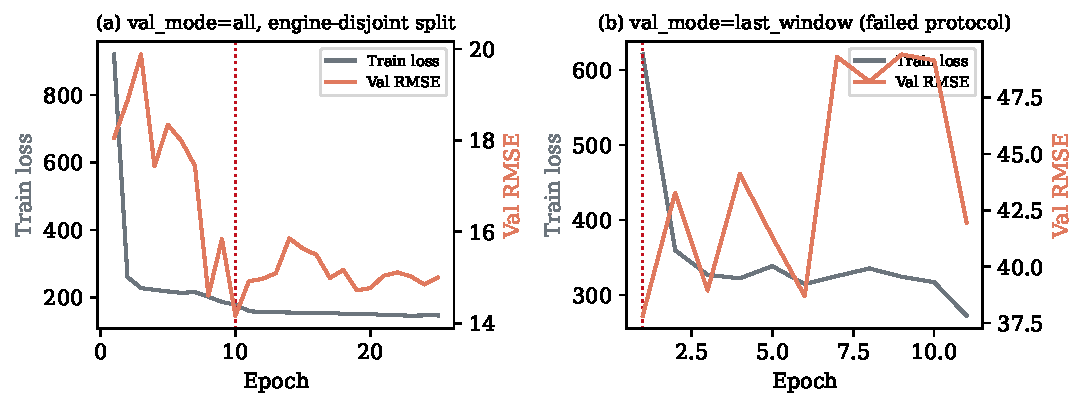
\includegraphics[width=\linewidth]{fig6_training_curves.pdf}
  \caption{FD001 training dynamics: correct vs.\ last-window validation (early stop at epoch 1).}
  \label{fig:train}
\end{figure}

Figure~\ref{fig:train} shows how the validation protocol affects training: last-window validation locks an underfit checkpoint at epoch 1.

%==============================================================================
\section{Conclusion}
%==============================================================================

This report delivers an end-to-end GPT4RUL reproduction on C-MAPSS with 12+ diagnostic experiments, highlighting methodological pitfalls in LLM-based PHM.
Main outcomes:
\begin{enumerate}
  \item Reproducible open-source pipeline with one-click scripts (\texttt{reproduce.ps1}).
  \item Best current result: Hybrid+Soft Prompt on FD002 (RMSE 12.55).
  \item Engine-disjoint splits and full validation windows are necessary for credible evaluation.
\end{enumerate}

\textbf{Recommendations:} always split by engine ID; never validate on last-window-only subsets; encode operating conditions for multi-regime data.
Future work: GPT-2 layer ablation, multi-seed reporting, and fully logged paired ablations.

\vspace{0.3em}
\noindent\textbf{Repository:} \url{https://github.com/icemilk-1/GPT4RUL-Reproduction}

\end{document}
